\documentclass[]{article}
\usepackage[T1]{fontenc}
\usepackage[utf8]{inputenc}
\usepackage[french]{babel}
\usepackage[]{graphicx}
\usepackage[]{hyperref}

\title{Bilan de projet}
\author{
    Théo DELMAS\\
    Lauric TEYSSEYRE\\
    Pierre-Louis RENON\\
    Julien WATTIER\\
    \\
    Université Paul Sabatier\\
    Master Informatique 1\\
   } 

\begin{document}
\maketitle
\newpage
\tableofcontents
\newpage

\begin{section}{Objectif du document}
 Ce document présente le bilan du projet.
\end{section}

{
\setlength{\parindent}{0pt} %Retire les alinéas
\begin{section}{Référentiel initial}
 Le référentiel initial est disponible à \href{https://github.com/Szyckaa/UE-PROJET-DOCS-GESTION/releases/tag/2.0.0}{cette adresse}.
 Le plus simple est de récupérer tous les PDF dans un dossier, et de placer les registres dans un sous-dossier "documents" afin de rendre les hyperliens du plan de projet valide.
\end{section}

\begin{section}{État courant à la terminaison}
 \begin{subsection}{Produits réalisés}
     L’état des produits à la terminaison du projet est exposé dans le schéma ci-dessous. Le code couleur indique leur état selon le code suivant :

     \begin{itemize}
         \item Vert : le produit a été réalisé.
         \item Jaune : le produit va être réalisé.
         \item Rouge : le produit n’a pas été réalisé.
     \end{itemize}

     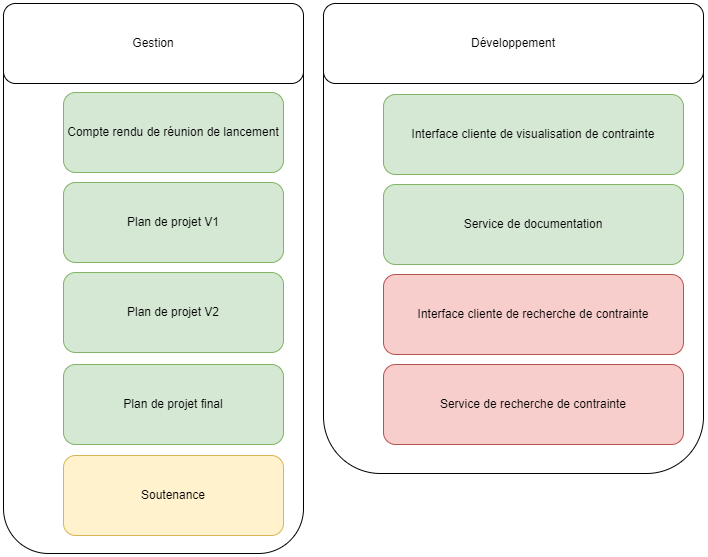
\includegraphics[scale=0.49]{IMG/PBS_final}

     La soutenance va être produite après livraison de la dernière version du plan de projet. Cette dernière étant fixée au 16/03/2023.

     Concernant les produits liés au système de recherche de contraintes, il a été décidé début mars et avec accord du client qu’ils ne seraient pas produits faute de temps.
 \end{subsection}

 \begin{subsection}{Listes des événements}
     Le \href{Registre_des_faits_marquants.pdf}{registre des faits marquants} référence l'ensemble des événements ayant affecté le projet.
 \end{subsection}

 \begin{subsection}{Listes des décisions}
     Conformément à la gestion des décisions du plan de projet, le \href{Registre_des_décisions.pdf}{registre des décisions} référence l'ensemble des décisions ayant amendé le plan de projet.
 \end{subsection}

 \begin{subsection}{Listes des livrables de gestion}
     L'ensemble des livrables de gestion est disponible sur ce \href{https://github.com/Szyckaa/UE-PROJET-DOCS-GESTION}{dépôt github}, en consultant les releases.
 \end{subsection}

 \begin{subsection}{Listes des livrables de développement}
     L'ensemble des livrables de développement est disponible sur le \href{https://framagit.org/flopedt/FlOpEDT}{dépôt framagit du projet}. Conformément à notre gestion des livrables, ces derniers sont intégrés dans la \href{https://framagit.org/flopedt/FlOpEDT/-/tree/catalog}{branche catalog}.
 \end{subsection}
\end{section}

\begin{section}{Analyse du déroulement du projet}
 \begin{subsection}{bilan technique}
     \begin{subsubsection}{Un contexte difficile}
         Pour rappel le projet dans sa globalité est en train de découpler son back, réalisé avec Django, de son front qui jusque-là était géré également par Django pour migrer vers VueJS. Dans ce contexte le client nous a demandé de réaliser les nouvelles fonctionnalités en utilisant les nouvelles technologies.

         Malheureusement cela a été compliqué car les fonctionnalités développées reposent sur du code existant qui n'utilise pas VueJS. Il a donc fallu mettre en place divers mécanismes pour s'intégrer sur l'existant.
     \end{subsubsection}

     \begin{subsubsection}{L'installation de l'environnement de travail compliquée}
         L'équipe a eu de nombreuses difficultés pour installer le serveur de développement car elle pensait pouvoir utiliser Docker mais il s'est révélé que le projet ne maintenait plus le nécessaire pour fonctionner dessus.

         Par la suite, elle a eu quelques problèmes car une partie des développeurs utilisaient WSL plutôt qu'une vraie machine virtuelle pour le serveur.

         Tout cela a rendu le sprint 0 plus long en faisant perdre plusieurs jours de travail et donc au projet.
     \end{subsubsection}

     \begin{subsubsection}{Une connaissance préalable des technologies imposées }
         L'équipe avait une bonne expérience avec le framework front-end VueJS ; imposé dans ce projet ; de par les cours dispensés à l'université et de par des expériences professionnelles pour certains des développeurs.

         Cela a été utile pour l'intégration sur l'existant.
     \end{subsubsection}

     \begin{subsubsection}{Une équipe aux affinités techniques variées }
         D'autre part l'équipe a eu la chance de ne pas avoir de problème pour savoir qui se chargerait du front ou du back puisque rapidement les développeurs se sont mis d'accord selon leurs affinités. Cela a évité de travailler à contre-coeur sur une technologie et donc de faire perdre du moral à l'équipe.
     \end{subsubsection}

     \begin{subsubsection}{Conclusion sur l'aspect technique}
        D'un point de vue technique, le projet c'est plutôt bien déroulé malgré un contexte et un départ difficile.
     \end{subsubsection}
 \end{subsection}

 \begin{subsection}{Bilan méthodologique}
     \begin{subsubsection}{L'analyse de l'existant négligée}
         Au milieu du projet l'équipe a appris que le projet dans sa globalité utilisait une convention consistant à partir du principe que si une liste d'objets du système est vide c'est qu'en réalité elle désigne toutes les instances de la classe de ces objets.

         Si l'adaptation ne nous a pas posés de problèmes, cela révèle que nous n'avions pas une connaissance suffisante des systèmes impactés par notre travail car nous n'avons pas pris le temps de les analyser avant de commencer les développements.
     \end{subsubsection}

     \begin{subsubsection}{Un manque de contrôle}
         L'équipe n'a appliqué presque aucun contrôle des activités ou des produits.

         D'une part aucun processus clairement défini n'a été mis en place afin de contrôler les différentes activités du projet. Et d'autre part l'équipe n'a produit aucun indicateur permettant d'évaluer les activités et produits du projet. De fait elle ne pouvait pas sérieusement contrôler en se basant sur les variations des indicateurs.

         La principale conséquence est que faute de moyens pour visualiser quantitativement la qualité des différentes activités et produits, la qualité de manière générale n'a que peu de sens dans ce projet. D'autre part l'absence d'activité de contrôle peut provoquer une déviation du projet sans que l'équipe ne s'en rende compte, ou trop tard, impactant énormément le projet.
     \end{subsubsection}

     \begin{subsubsection}{Peu de conception}
         L'équipe n'a pas suffisamment insisté sur les phases de conception et avait tendance à directement expérimenter des solutions en codant plutôt qu'en analysant le problème et en modélisant des solutions.

         L'équipe à certainement manqué de recul et donc réduit la qualité des produits.
     \end{subsubsection}

     \begin{subsubsection}{L'évolution de la gestion}
         Il faut savoir que nous avons commencé le projet sans avoir de plan de projet, ni de connaissances sur la gestion de projet. De fait nous avons dû élaborer les règles et processus au fur et à mesure, et donc changer nos méthodes de travail.

         Cela nous a grandement impacté car nous avons régulièrement pris conscience que certains processus auraient dû être appliqués dès le début du projet, créant une certaines frustration impactant le moral.
     \end{subsubsection}

     \begin{subsubsection}{Une gestion du besoin initialement trop faible}
         Au début du projet l'équipe ne produisait pas de rapport de réunion mettant en relief les actions à effectuer pour le projet. De fait, les tâches à effectuer n'étaient pas forcément mises à jour dans l'immédiat et certaines ont été temporairement oubliées.

         Cela n'a que peu impacté le projet car les tâches oubliées n'étaient pas prioritaires mais cela aurait pu grandement impacter les artefacts produits en créant une différence entre ce qu'attendait le client et ce que produisait l'équipe.
     \end{subsubsection}

     \begin{subsubsection}{Aucune définition du protocole de traitement des besoins et du test}
         L'équipe n'a jamais défini un protocole de traitement des besoins précisant qu'elle devait s'assurer qu'un besoin passe en "Ok" (Done) avant d'en traiter un autre étant en "A faire". Elle s'est permis d'enchaîner la réalisation des besoins sans les tester, persuadée qu'elle pourrait le faire vers la fin du projet. Elle a donc accumulée une forte dette technique qu'elle n'a pu rattraper dans les temps.

         D'autre part elle n'a pas défini le protocole de test dès le début, encore une fois persuadée qu'elle pourrait le faire sur la fin du projet, ce qui l'a incité à enchaîner la réalisation sans tester, et donc à accumuler de la dette technique.
     \end{subsubsection}

     \begin{subsubsection}{Des communications efficaces}
         L'ensemble des communications à globalement bien été géré.

         D'une part les communications internes ; qui consistaient à avoir l'ensemble des fournisseurs en vocal sur discord ; ont permis un développement efficace puisqu'en cas de problème, un développeur était immédiatement aidé. Cela a également fortement augmenté la cohésion de l'équipe qui malgré la distance était toujours en contact.

         Concernant les communications avec le client, elles se faisaient essentiellement lors des revues de sprint qui étaient tenues toutes les deux semaines, ce qui s'est révélé être un bon rythme au vu du projet, permettant de s'assurer de la conformité entre les besoins du client et la réalisation. Ce dernier était également très disponible pour des discussions plus informelles qui permettaient d'affiner rapidement des besoins s'étant révélés trop flous.
     \end{subsubsection}

     \begin{subsubsection}{Conclusion sur l'aspect méthodologique}
        Avec le recul, l'équipe se rend compte qu'elle manquait de méthodologie. Le projet a été validé par le client qui semble satisfait mais ce manque de rigueur aurait très bien pu mettre en échec le projet.
     \end{subsubsection}
 \end{subsection}
\end{section}

\begin{section}{Leçons apprises}
 \begin{subsection}{L'importance de la phase d'initialisation du projet}
     La phase d'initialisation est l'occasion de définir rigoureusement les différents processus et règles appliqués par l'équipe. Cette base évoluant par la suite selon les besoins. Dans de véritables projets, avoir un définition initiale rigoureuse nous semble essentielle pour la bonne conduite du projet.

     Dans le cas de projet d'extension, c'est durant cette phase que l'équipe chargée de la réalisation devrait s'imprégner du projet à modifier en comprenant comment fonctionnent les différents systèmes qui vont être impactés.
 \end{subsection}

 \begin{subsection}{L'importance du contrôle}
     Le contrôle permet d'assurer la qualité du projet en analysant des indicateurs pertinents qui sont produits tout au long du projet.

     Il nous paraît évident que ces processus auraient ajouté une plus-value au projet en nous permettant de l'évaluer quantitativement, et donc prendre des décisions pertinentes au regard des résultats des analyses. Cette classe de processus n'est donc pas à négliger.
 \end{subsection}

 \begin{subsection}{L'importance des communications}
     La forte communication avec le client semble être un point plus que bénéfique dans le cadre des projets agiles afin de valider l'adéquation entre un besoin et sa réalisation. 

     Concernant les communications internes, elles ont eu un double intérêt dans ce projet puisqu'elles ont renforcé la cohésion de l'équipe tout en évitant les situations de blocages des développeurs.
 \end{subsection}
\end{section}

\begin{section}{Perspectives}
 \begin{subsection}{Insister sur la conception}
     En maintenant des schémas UML des productions et de l'existant impacté, l'équipe pourrait bénéficier d'une vision globale du problème au moment de réaliser les tâches. De là, elle pourrait ainsi modéliser diverses solutions et sélectionner celle respectant au mieux nos exigences. Les développements des fonctionnalités seraient certainement plus efficaces ainsi.
 \end{subsection}

 \begin{subsection}{Définition rigoureuse du traitement des besoins}
     En définissant dès le départ un protocole de traitement des besoins qui minimise l'accumulation de dette technique, l'équipe pourrait produire des artéfacts de meilleure qualité. Dans le cadre de ce projet, ce protocole aurait dû spécifier qu'il était interdit de traiter un nouveau besoin dans que celui actuellement traité ne devenait pas "Done", et donc au passage bien définir "Done". Ainsi il n'y aurait pas eu d'absence de test et donc une telle dette technique.
 \end{subsection}

 \begin{subsection}{Appliquer du contrôle}
     L'équipe devrait produire dès le début des indicateurs qui seraient maintenus à jour durant tout le projet. L'intérêt serait double : d'une part, se rendre compte si un des aspects du projet dévie. D'autre part, permettre l'optimisation du fonctionnement de l'équipe en prenant des décisions rationnelles basées sur ces indicateurs.
 \end{subsection}
\end{section}

\begin{section}{Recommandations}
 \begin{subsection}{Migrer avant d'étendre}
     Pour rappel l'application est actuellement en train de migrer d'une application monolithique Django vers un front VueJS et un back Django dissocié. Notre travail consistait à étendre l'application en ajoutant un système. Au vu du contexte le client souhaitait que les nouveaux développements respectent la nouvelle philosophie de front et back dissociés.

     Malheureusement cela a rendu nos développements compliqués en nous forçant à nous adapter à un code qui est voué à disparaître, notamment côté front. Nous pensons donc que la migration devrait être effectuée ; ou du moins bien entamée ; avant de réaliser de nouvelles extensions.
 \end{subsection}

 \begin{subsection}{Documentation du code source}
     L'équipe qui maintient le projet devrait mettre en place une documentation assez généraliste qui décrit ce que chaque partie du projet réalise en ajoutant des markdowns dans les différents dossiers du projet. Cette documentation semble essentielle sachant que le projet est open source et que son absence de documentation est un frein pour les nouveaux arrivants.
 \end{subsection}
\end{section}

}
\end{document}